\documentclass[12pt]{article}

\usepackage{parskip}
\usepackage[margin=2.7cm,a4paper]{geometry} % Page formatting
\usepackage{multicol} % For multi-column sections
\usepackage{graphicx} % For including images
\usepackage{url}
\graphicspath{ {./images/} }
\usepackage{amsmath,amsthm,amsfonts,amssymb,mathtools} % For math symbols

% Math config
\DeclarePairedDelimiter\ceil{\lceil}{\rceil}
\DeclarePairedDelimiter\abs{\lvert}{\rvert}
\DeclarePairedDelimiter\set{\{}{\}}

% Header
\usepackage{fancyhdr}
\addtolength{\headheight}{2.5pt}
\pagestyle{fancy}
\fancyhead{} 
\fancyhead[L]{\sc INFO2222}
\fancyhead[C]{\sc bkni0201, kwal3204}
\fancyhead[R]{Project part 2: Usability}
\renewcommand{\headrulewidth}{0.75pt}

\usepackage[noend]{algpseudocode} % Pseudocode
\usepackage[tikz]{mdframed} % Outlined pseudocode

\newcommand{\bryce}{\hfill\normalsize\sc [bkni0201]}
\newcommand{\kai}{\hfill\normalsize\sc [kwal3204]}

\newcommand{\ekey}{\textsc{exchangeKey} }
\newcommand{\rkey}{\textsc{roomKey} }
\newcommand{\skey}{\textsc{storageKey} }

\newcommand{\func}[1]{\textsc{#1()}}

\begin{document}

\tableofcontents
\newpage

\section{Relation To Security Project}

Before beginning this stage of the project, there were some issues in the previous stage that we addressed at the beginning:

\textbf{The application breaks web crypto API specifications.} Upon login, we use \func{importKey} to import the user's password as a base cryptographic key, from which we derive \skey (described in the security project report). When importing this, the base key material was unnecessarily set \texttt{extractable=true}, which goes against the API specifications, but only caused an error in Google Chrome, rendering the application unusable. This was an easy fix, setting \texttt{extractable=false}.


\section{User Investigation}

\textbf{TODO in this section:}
\begin{itemize}
    \item Choose a user group, Students OR Alumni OR administrators
    \item Perform a PACT analysis on the chosen group
    \item Perform research on user group (surveys/interviews)
    \item Create a persona document for the user group
    \item Gather content of interest to target persona to be used for knowledgebase functionality examples (documents, articles)
\end{itemize}

\section{Design Plan} % Navigation Design in specs

\textbf{TODO in this section:}
\begin{itemize}
    \item Create "wishlist" of features
    \item conduct card-sorting with target users
    \item *maybe* since card sorting is for parts of the overall site, a section here for site-wide usability changes
    \item Outline results in report
    \item Using results, create a sitemap
\end{itemize}

\section[Prototype]{Prototype}

\textbf{TODO in this section:}
\begin{itemize}
    \item Using gathered information, brainstorm and create sketches of designs
    \item Create a prototype from the best design
    \item Perform a guerilla test, including group members and an outside person
    \item Outline guerilla test, including findings
    \item Make improvements to design plan from test findings
\end{itemize}

\section[Implementation]{Implementation Of Prototype}

\begin{itemize}
    \item Incremental Development Plan, each iteration 2 weeks
    \item Outline evaluations conducted
    \item Demonstrate functionality
    \item Self-evaluate, including team contribution
\end{itemize}

\subsection{META: Independent Features To Implement}

Due to the security project taking longer than expected, and the 1 week extension delaying its completion further, we simply didn't have enough time to wait for the design process to be completed before implementing new things. Following is a hastily made list of features and changes we were able to make to our code, independently of the results of the design process. These changes are either straight from the assignment specifications, or general web-development best practices.

\begin{itemize}
    \item New database table for articles
    \begin{itemize}
        \item Title, blurb, content attributes
        \item Comments go in new pooled database, with reference to article ID for easy modification
        \item Ensure proper content formatting, markdown, html, no XSS
        \item Database functions to edit, remove articles and comments
    \end{itemize}
    \item Implement architecture for multi-user chatrooms
    \begin{itemize}
        \item Rooms need to be decoupled from friendship id
        \item First 2 users perform exchange, agree on roomkey. each subsequent user generates an RSA pair and requests the room key.
        \item If we use RSA-OAEP from web crypto API, we get message integrity.
    \end{itemize}
    \item Implement staff ability to mute user from room or article (specs are unclear on exact meaning)
    \item New attributes for users, rank (student, staff, admin)
    \item List of online users (in python code, not database)
    \item HTML and CSS best practices
    \begin{itemize}
        \item Semantic html (main, nav, section, header instead of divs)
        \item Appropriate use of forms to enclose inputs
        \item label form inputs (helps people using screen readers)
        \item Ensure proper text formatting, size, tontrast (rems fopr sizing)
        \item Color code buttons for positive, negative, passive actions (e.g. green, gray, red)
        \item Add listeners for key presses, like enter on password entry
    \end{itemize}
\end{itemize}

\newpage
\section{DELETE THIS SECTION: Example code}

\begin{figure}[h]
    \caption{This is an example figure}
    \centering
    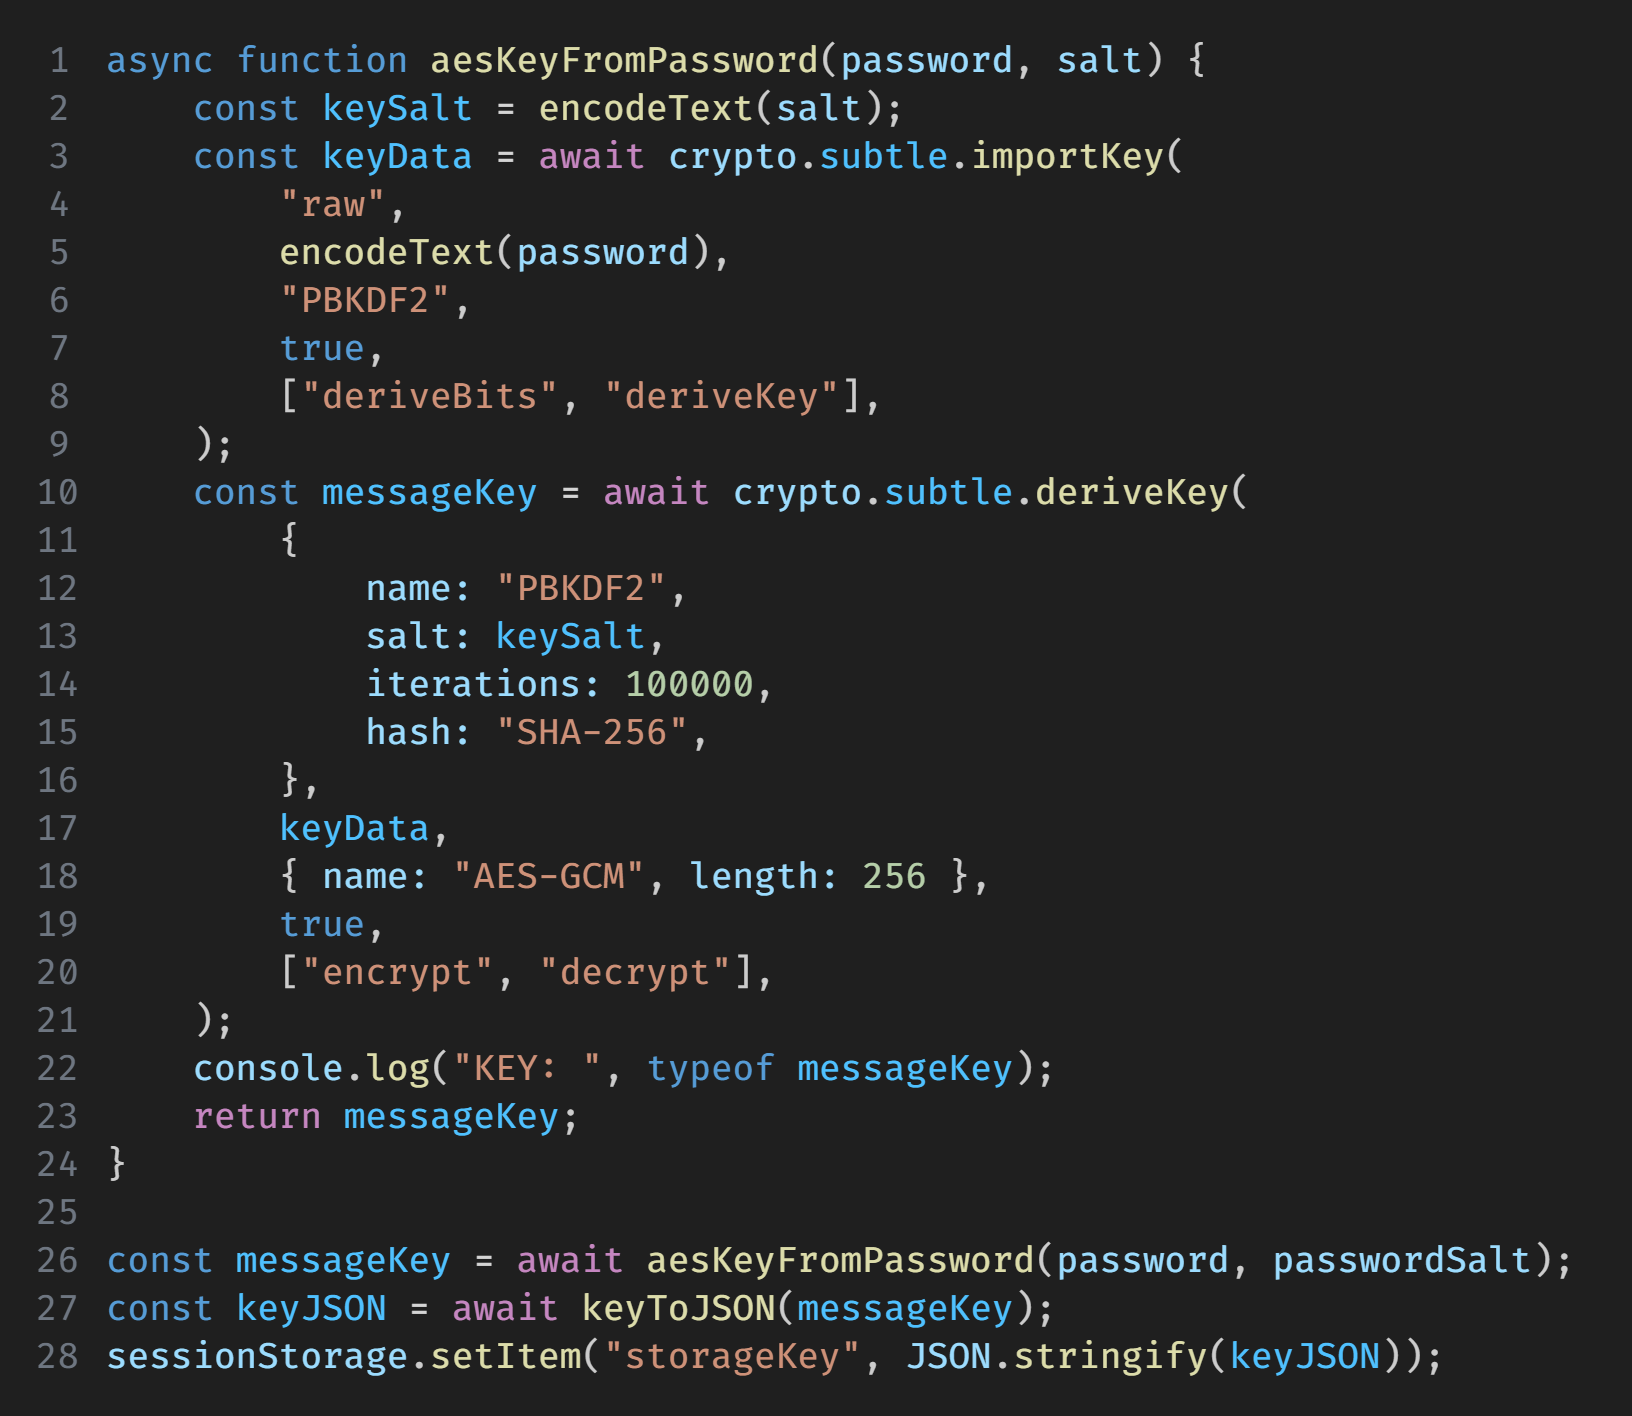
\includegraphics[width=0.75\textwidth]{oldAesFromPassword.png}
\end{figure}

This figure was generated using the codesnap \cite{CodeSnap} vscode extension, with the following settings in \texttt{settings.json}

\begin{verbatim}
"codesnap.showWindowControls": false,
"codesnap.containerPadding": "0",
"codesnap.roundedCorners": false,
"codesnap.boxShadow": "none"
\end{verbatim}

\bibliographystyle{ieeetr}
\bibliography{refs}

\end{document}

